\documentclass{article}
\usepackage{biblatex} %Imports biblatex package
\addbibresource{ref.bib} %Import the bibliography file
\usepackage{titling}
\usepackage{titlesec}
\usepackage{caption}

\titleformat{\subsection}[runin]
  {\normalfont\large\bfseries}{\thesubsection}{1em}{}
% commands
\DefineBibliographyStrings{english}{%
    andothers = {\em et\addabbrvspace al\adddot}
}
 
 
\setlength{\droptitle}{-15em}   % This is your set screw
\usepackage[utf8]{inputenc}
\usepackage[hashEnumerators,smartEllipses]{markdown}
\title{An Exploration of ECG Pre-processing Techniques}
\author{Amir Salimi \and Ali Naeim Abadi}


\begin{document}

\maketitle

% \section{Background }

% Time series are a type of data where the data points are listed chronologically in time. ECG signals contain multiple 1 dimensional time series called channels or leads.  Typically, an ECG signal is a recording of several parts of the cardio vascular system, each sensor recording 1 lead. Typically, ECGs contain 12 leads, and ECG technicians can diagnose heart conditions by looking at the ECG recording of a patient and finding abnormalities in 1 or more of the leads. 
% The first sentence of an abstract should clearly introduce the topic of the paper so that readers can relate it to other work they are familiar with. However, an analysis of abstracts across a range of fields show that few follow this advice, nor do they take the opportunity to summarize previous work in their second sentence. A central issue is the lack of structure in standard advice on abstract writing, so most authors don’t realize the third sentence should point out the deficiencies of this existing research. To solve this problem, we describe a technique that structures the entire abstract around a set of six sentences, each of which has a specific role, so that by the end of the first four sentences you have introduced the idea fully. This structure then allows you to use the fifth sentence to elaborate a little on the research, explain how it works, and talk about the various ways that you have applied it, for example to teach generations of new graduate students how to write clearly. This technique is helpful because it clarifies your thinking and leads to a final sentence that summarizes why your research matters.
\begin{abstract}
Are there any best practices when it comes to pre-processing of Electrocardiogram (ECG) signals for automatic diagnosis of heart disease? 
State of the art machine learning algorithms have achieved remarkable results by learning from multi-lead ECG signals, yet rarely is the pre-processing and augmentation decisions for training these models justified or the effect of their absence measured. Understandably, discerning such rules is difficult since different datasets, diseases, and model architectures may require different pre-processings steps for optimal performance; in addition, the sheer number of methods and parameters which need to be explored can be overwhelming. Here, we study the interaction between different machine learning (ML) models, different multi-label ECG datasets, and several commonly used pre-processing and augmentation techniques for classification of heart disease. We look for reliable, simple to implement techniques which are agnostic to specific model architectures, datasets, and diseases. Our work can be easily replicated and expanded by those interested in model architectures or signal transformations. We hope that the methods explored here will remain beneficial to future researchers as more architectures and datasets are discovered and made available. 


\end{abstract} \hspace{12pt}
\section{Introduction and Problem Definition}
Researchers must make many decisions and guesses before deploying machine learning models for classification of heart disease using ECG data. Many of these decisions regarding pre-processing of data, length and amount of data needed, and purpose of model (multi-label vs single label) do no yet have clear answers. Here we combine different models with different ECG datasets and data processing approaches. We seek to either find concrete answers to these problems, or narrow the range of possible options. 

State of the art algorithms in diagnosis of heart disease have achieved remarkable results by learning from raw 12-lead ECG signals~\cite{reyna2021will,reyna4issues}. However, these algorithms generally require tens of thousands of examples and long training times to achieve peak performance~\cite{reyna2021will,reyna4issues,natarajan2020wide}. Such large datasets require thousands of hours of manual recording and labeling and may not be available for less common heart conditions. Several factors can interfere with the recording process and add noise to the ECG. These include noise from activity of muscles unrelated to the cardiovascular system as well as baseline wonder and powerline interference~\cite{sornmo2006electrocardiogram}. It is common for these ECG signals to go through a pre-processing step before to remove unnecessary data from the ECG signal before it is analysed or given to a machine learning algorithm~\cite{gacek2011ecg,sornmo2006electrocardiogram}. An analysis of the top performing submissions the Physionet2020 ECG classification challange shows that many of the teams employed such methods to further process and augment raw ECG files.

Here, we define~\textit{pre-processing} as any function which modifies the original signal in order to increase model performance, decrease training times, or training of bigger models without increasing computational demand. Examples of pre-processing functions are~\textit{band-pass filters}, which remove un-necessary frequencies from the signals and~\textit{down-sampling}, which decreases signal resolution but reduces computing requirements.  We define~\textit{augmentation functions} as a subset of pre-processing functions which aim to deal with the issue of limited data, such as adding noise or cutting out parts of data during training times.

While these methods are commonly used by state of the art models, rarely is any justification given for their parameters and the performance of these models with and without pre-processing is not explored. In addition, some of the top performing algorithms apply minimal processing to the signals~\cite{natarajan2020wide,ribeiro2020automatic}. This lack of best practices is understandable as there are a wide variety of choices to be made in the machine learning pipeline; researchers must account for several factors which may interact with the others in unexpected ways: the pre-processing transformations applied to the data, the model hyper-parameters, the heart disease(s) of interest, and whether the model is classifying single or multiple labels. Such a through analysis of all possible combinations and parameters can be overwhelming and unfeasible for most researchers both from a time and computation persepective. Furthermore, there is no guarantee that a learning pipeline which is optimal for one dataset and/or heart disease to be effective on other datasets or diseases. 

In this work we are looking for general best practices which can be helpful to as many future works as possible. Rather than strictly attempting to set new performance benchmarks, the goal here is to observe the effect of common pre-processing and augmentation functions when applied to different datasets of ECGs containing different heart diseases. We employ different state of the art time-series classification models, and measure the effectiveness of the various combinations in order to see if we can find any general rules towards automatic classification of heart disease.

\begin{table}[tpb]
\centering
\begin{tabular}{|c|c|}
 \hline
Label & Count \\
 \hline
right bundle branch block    &  1857 \\
ventricular ectopics         &   700 \\
atrial fibrillation          &  1221 \\
1st degree av block          &   722 \\
premature atrial contraction &   616 \\
sinus rhythm                 &   918 \\
st depression                &   869 \\
 \hline
\textbf{Total} & \textbf{6903}\\
\hline
\end{tabular}
% (394, 368, 6903)
\caption {\textbf{CPSC2018} dataset of 6877 ECGs. 368 ECGs have no labels. 394 ECGs have more than 1 label.\\}
\label{tab:CSPC}

\begin{tabular}{|c|c|}
 \hline
Label & Count \\
 \hline
left ventricular high voltage &  1295 \\
atrial fibrillation           &  1780 \\
t wave abnormal               &  1876 \\
sinus bradycardia             &  3889 \\
supraventricular tachycardia  &   587 \\
sinus rhythm                  &  1826 \\
sinus tachycardia             &  1568 \\
nonspecific st t abnormality  &  1158 \\
 \hline
\textbf{Total} & \textbf{13979}\\
\hline


\end{tabular}

\caption {\textbf{Chapman-Shaoxing} dataset of 10247 ECGs. We drop labels that appear in less than 5\% of the ECGs. 337 ECGs have no labels. 3334 ECGs have more than 1 label.}
\label{tab:ChapmanShaoxing}
        % from zhang et al We recommended a low-frequency flter to cut of 0.67Hz or below with zero phase distortion, and ahigh-frequency flter with 50Hz cutof frequency. Using the raw ECG signal is also an option for classifcation scheme.

\end{table}

\section{Datasets}
\label{datasets}
We conduct our experiments on two datasets, the~\textbf{CSPC} dataset~\cite{liu2018open} and the \textbf{Chapman-Shaoxing} dataset~\cite{zheng202012}. Both of these datasets have been released as part of the 8 datasets of labeled 12 lead ECGs provided by the Physionet\-2021 challenge~\cite{reyna2021will,reyna4issues}. We will initially focus on the CSPC datset, released as part of the ICBEB-2018 competition~\cite{liu2018open} and implement a model which can match the results of the competition winner before moving on to measuring pre-processing effects. We use the Chapman-Shaoxing dataset~\cite{zheng202012} as our secondary dataset to verify our findings. The breakdown of these datasets and their label counts is given in Tables~\ref{tab:CSPC} and ~\ref{tab:ChapmanShaoxing}.

\section{Models}
\label{sec:models}
We use two models with proven results in state of the art time-series classification tasks: the Inception-Time Network, which is the 1-dimensional application of the Inception-Network~\cite{szegedy2017inception,ismail2020inceptiontime} and MiniRocket, a quick and mostly deterministic feature extractor for time-series~\cite{dempster2021minirocket}. A recent survey of time-series classification methods by Ruiz~\textit{et al.} highlights both of these models as excellent performers in various multi-variable time-series classification benchmarks. In the context of ECG classification, Inception-Time has achieved state of the art performance ECG classification tasks~\cite{Strodthoff2021}. 


\section{Pre-Processing And Augmentation}
\label{sec:processing}
\begin{table}[tpb]
\centering
\begin{tabular}{lll}

Rank &                                                                 Data preprocessing &                                                                          Data augmentation \\
                                             \\
1    &  500Hz;\ Bandwidth 3 - 45 Hz; Value -1 - 1; Window size 15s 0-padding &                                                                                         No \\
2    &                257 Hz; Value -1 - 1; Window size 4096(16s) 0-padding &                                                                                         No \\
3    &   500Hz; Window size 30s 0-padding; Exclude 4 leads; Wavelet denoise &                                                                  With external data: Hefei \\
4    &                     500Hz; Value -1 - 1; Window size 10240(20.48 s)  &                                                                        Add noise and drift \\
5    &                                              250Hz; Value normalized &  Add or filter frequency components; Substitute, shuffle, invert, filt and scale lead data \\
\end{tabular}
\caption{Top performing teams' approaches to ECG pre-processing and augmentation. Subset of the larger survey conducted by Hong~\textit{et al.}~\cite{hong2022practical}}
\label{tab:hong_top5}
\end{table}
A recent work by Hong~\textit{et al.} highlights the implementation decisions made by the successful submissions to the Physionet2020 ECG classification challenge~\cite{hong2022practical}. These decisions include length of input data, pre-processing and augmentation steps, model architectures, data-imbalance solutions, etc. From this survey, we see that there is a diverse set of decisions made by top performing teams in pre-processing and augmentation of ECG data before machine learning algorithms were applied. We higlight a subset of the decisions made by the top 5 performing teams in Table~\ref{tab:hong_top5}.  This survey does not narrow the range of viable options in pre-processing or augmentation since different teams used different architectures amongst other experiment inconsistencies. 

In this work we implement some of the most common approaches to augmentation and pre-processing as highlighted by Hong~\textit{et al.}~\cite{hong2022practical} and use ablation to observe their effects on different models and datasets. By doing so we'll be able to make more general statements about the effects of these methods on ECG signal classification and whether future researchers may or may not want to incorporate them into their own pipelines. 

% types of experiments
% un processed, normalized, scaled, bandpassed, shifted, all-together
\subsection{Normalization}
\subsection{Scaling}
\subsection{BandPass}
\subsection{Shifting}

\begin{table}[tpb]
\centering
\begin{tabular}{|l|l|l|l|}
\hline
Function      & Type         & Example Usages & Notes \\ \hline
Normalization & Pre-Process  &                &       \\ \hline
Scaling       & Pre-Process  &                &       \\ \hline
BandPass      & Pre-Process  &                &       \\ \hline
Shifting      & Augmentation &                &       \\ \hline

\end{tabular}
\caption{A list of processing and augmentation functions used. }
\label{tab:processing_funcs}
\end{table}

\section{ICBEB DataSet}
% do i cite this? results are bad but more recent: https://bmcmedinformdecismak.biomedcentral.com/articles/10.1186/s12911-021-01546-2
The ICBEB is an open access  released in 2018 as part a multi-label ECG classification competition~\cite{liu2018open}. ECG signal duration in this dataset is between 6 and 60 seconds, with an average duration of 15.79 seconds. The data the 12 leads were recorded at the frequency of 500 Hz. The entries to this competition trained on 6877 ECG recordings and were evaluated on a hidden test set of 2954 ECGs. To ensure our approach is competitive with the state of the art, we compare our results to the competition winner's reported F1 measurements after a 10 fold cross-validation on the training set where 80\% of the data was used for training and 10\% for validation, and 10\% for testing~\cite{chen2020detection}. Chen~\textit{et al.} reported the results for their best model, as well as an ensemble model of 130 models with various hyper-parameters.
We also compare our results to the more recent work by Strodthoff~\textit{et al.}~\cite{Strodthoff2021} who also used a 8/1/1 split for training, validation, and testing but only reported the average AUCs for their models. 

\subsection{InceptionTime}
\begin{figure}[!htbp]

  \makebox[\textwidth]{
    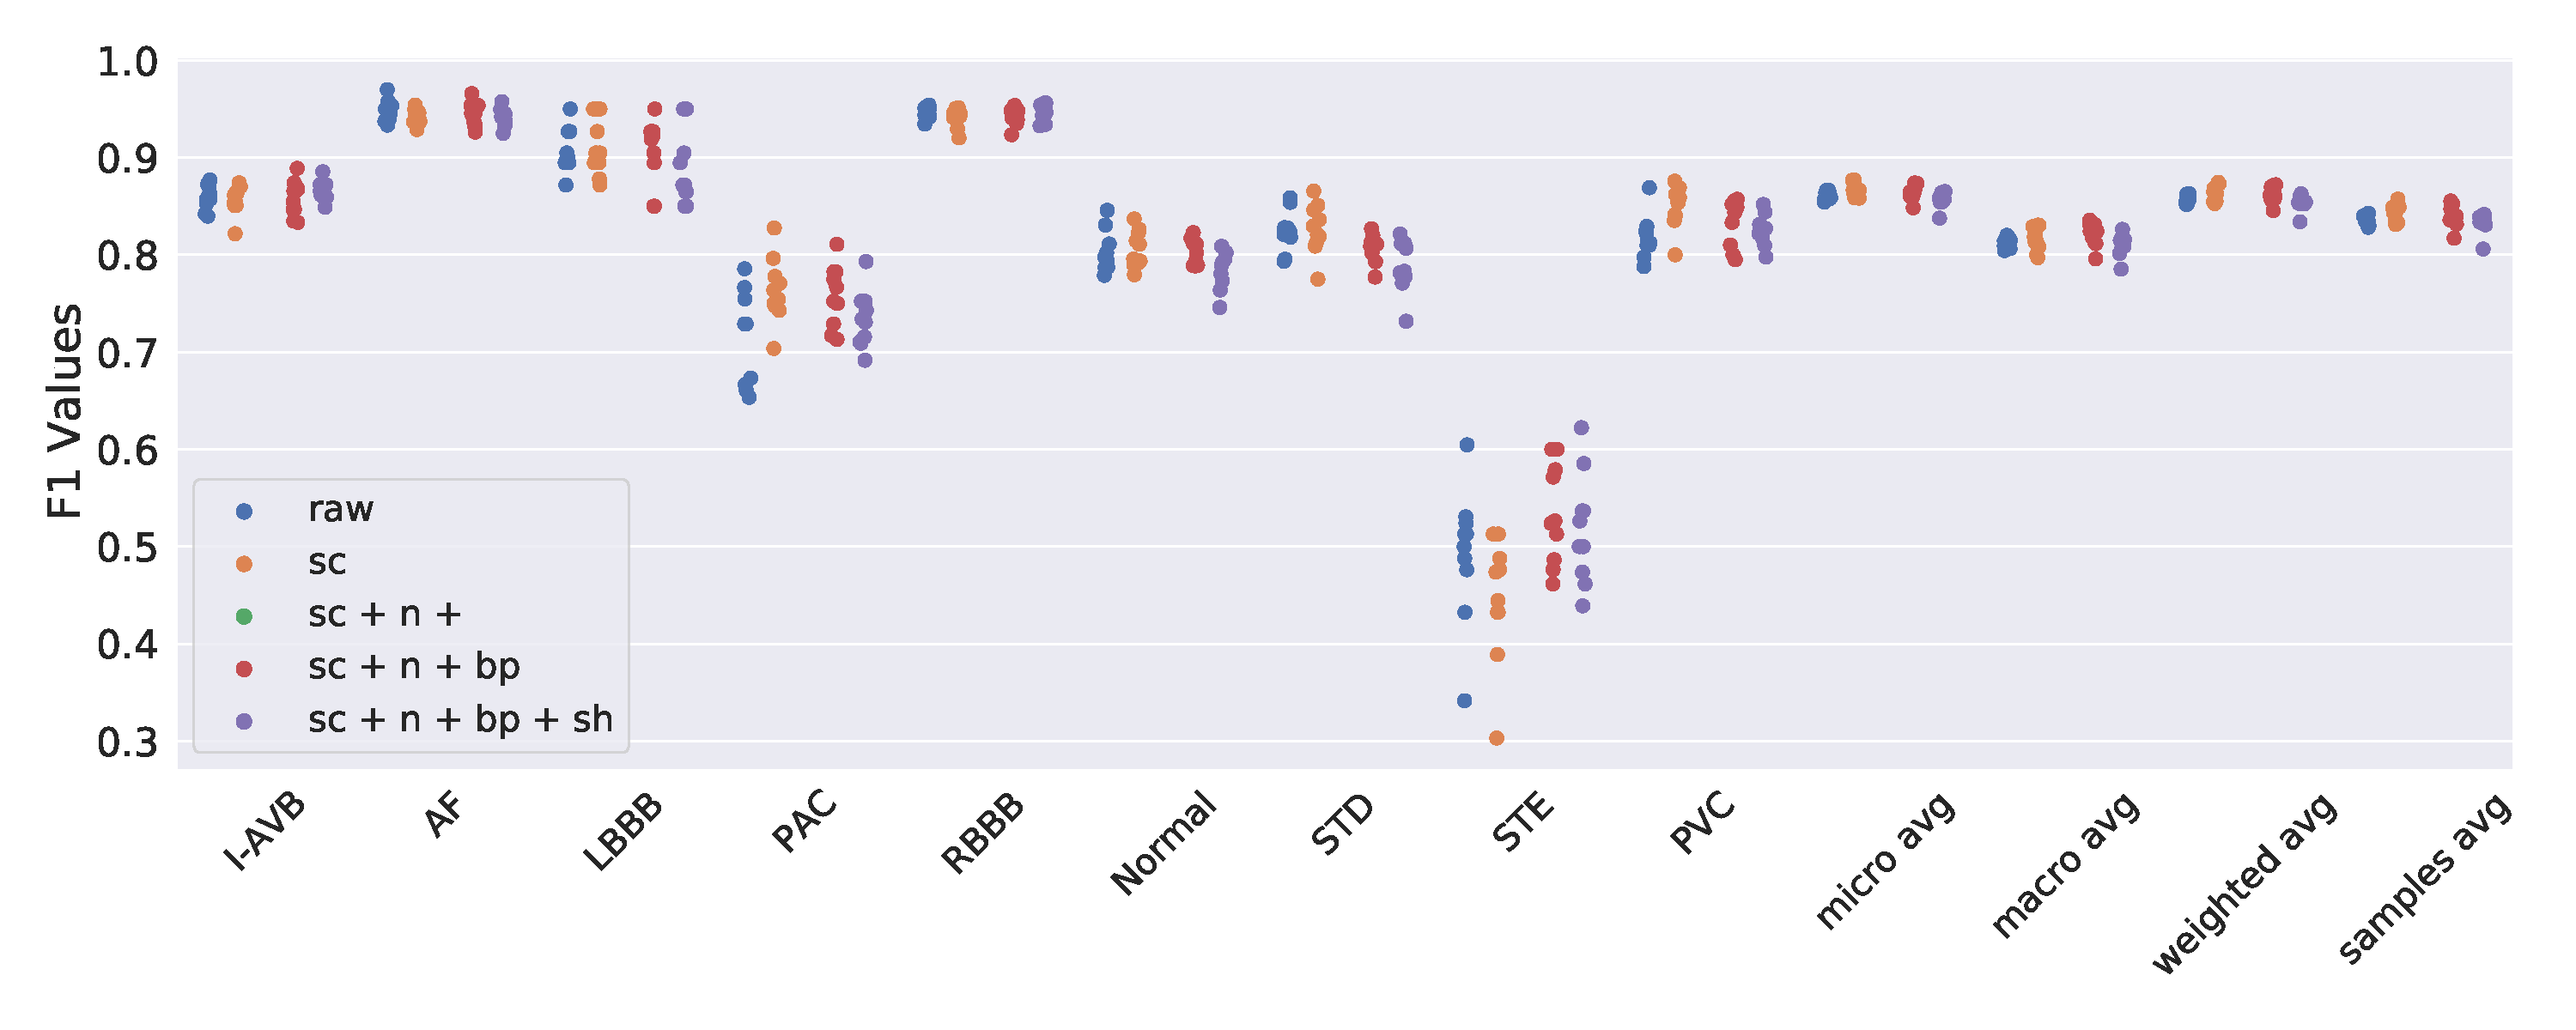
\includegraphics[width=\paperwidth]{images/inception_cpsc.pdf}
    
  }
  \caption{inception CPSC}\label{fig:inception_cpsc}
\end{figure}

\begin{table}[tpb]
\centering
\begin{tabular}{|cccccc|}
\hline

 &  raw &  sc &  sc-n &  sc-n-bp &  sc-n-bp-sh \\

1st degree av block          &                      0.860390 &                     0.858305 &                       0.861448 &                          0.860317 &                             0.867950 \\
atrial fibrillation          &                      0.947803 &                     0.941423 &                       0.942913 &                          0.945148 &                             0.943174 \\
left bundle branch block     &                      0.902381 &                     0.904762 &                       0.908907 &                          0.911840 &                             0.871795 \\
premature atrial contraction &                      0.728972 &                     0.759011 &                       0.751311 &                          0.759480 &                             0.732357 \\
right bundle branch block    &                      0.943734 &                     0.946015 &                       0.947505 &                          0.946151 &                             0.944941 \\
sinus rhythm                 &                      0.795646 &                     0.803255 &                       0.810050 &                          0.806625 &                             0.790428 \\
st depression                &                      0.824176 &                     0.825177 &                       0.810837 &                          0.810050 &                             0.782371 \\
st elevation                 &                      0.506410 &                     0.459064 &                       0.500000 &                          0.525063 &                             0.513158 \\
ventricular ectopics         &                      0.813246 &                     0.854540 &                       0.830926 &                          0.845929 &                             0.824623 \\
micro avg                    &                      0.861125 &                     0.865649 &                       0.861403 &                          0.863821 &                             0.857628 \\
macro avg                    &                      0.814593 &                     0.816061 &                       0.815315 &                          0.824211 &                             0.812525 \\
weighted avg                 &                      0.858318 &                     0.862641 &                       0.858093 &                          0.861098 &                             0.855021 \\
samples avg                  &                      0.834668 &                     0.844614 &                       0.839034 &                          0.838185 &                             0.834182 \\

\hline
\end{tabular}
\caption{Median of 10 fold cross-validation for inception model on the CSPC dataset}
\label{tab:inception_cspc}
\end{table}
\subsection{MiniRocket}
\begin{figure}[!htbp]

  \makebox[\textwidth]{
    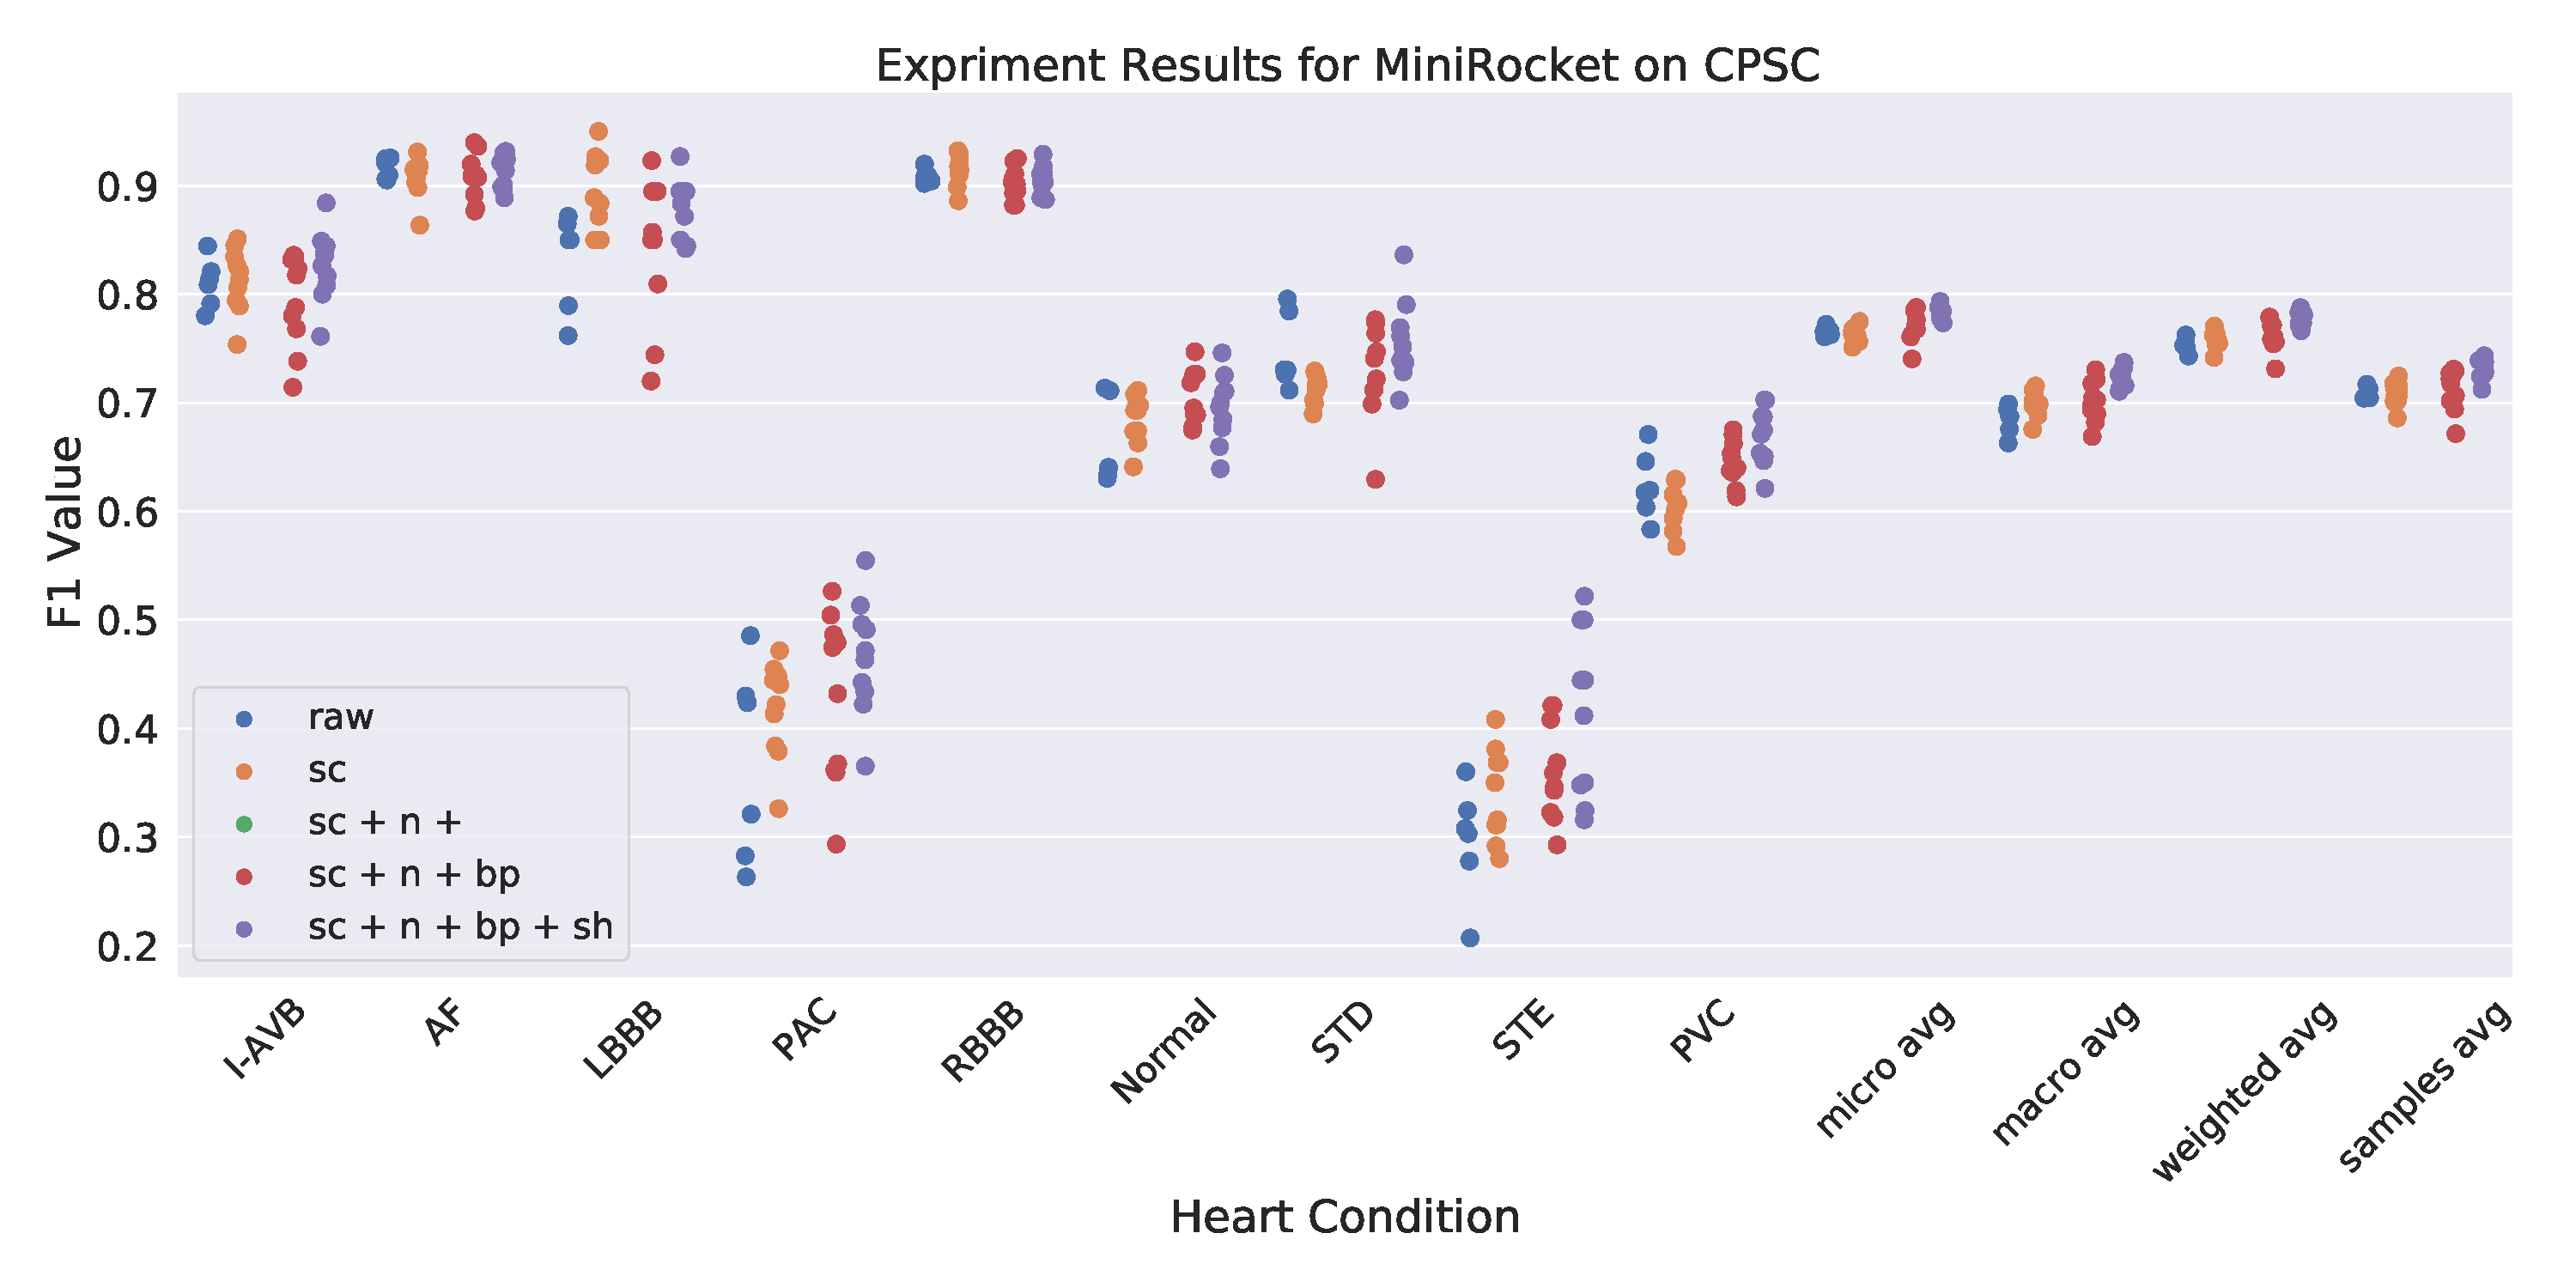
\includegraphics[width=\paperwidth]{images/mini_cpsc.pdf}
    
  }
  \caption{Mini CPSC}\label{fig:mini_cpsc}
\end{figure}
\section{Chapman-Shaoxing DataSet}
\subsection{InceptionTime}
\subsection{MiniRocket}

\section{Conclusion}
\printbibliography

\end{document}
